\section{\acrf{CBS}}
\label{sec:cbsAlgo}
As said \cbs is a two levels algorithm for solving the \acrs{MAPF} problem in a
correct and optimal way~\cite{MAPF_overview}. The work from Sharon et al. in
which \cbs was first proposed actually contains also a variant of the algorithm
to speed up cases in which two or more agents are frequently
colliding~\cite{CBS}. This variant is called \acrf{MACBS} and it merges the
agents that frequently conflict and considers them as a unique entity. This
though implies the fact that the low-level search must already be a \acrs{MAPF}
solver and not simply a \acrs{SAPF} solver. For this reason, this thesis
focuses on the classical version of \acrs{CBS}. \newline
We are going to first introduce two algorithms to solve the low-level search of
\cbs and then move to the description of the implementation of the high-level
search.
%
%
\subsection{Low-Level Search}
In \acrs{CBS}, the low-level search is the algorithm responsible for finding a
feasible path from an initial point to a final point on the graph for a single
agent. We shall distinguish two situations: the first call to the low-level is
for the creation of the root of the \acrl{ct}, while all the other calls are
for subsequent nodes. Each of the nodes, excluding the root, will have
constraints to abide to, and hence the low-level algorithm must be modified to
account for the presence of possible limitations. \newline 
Moreover, the majority of \acrs{SAPF} algorithms are one-shot in the sense that
they do not provide support for additional intermediate goals to reach. As
mentioned in Chapter~\ref{ch:introduction}, this thesis does not consider the
problem of mission planning, but only the motion planning one, this means that
we assume that the order in which the tasks are received is actually the best
one hence the problem focuses on to the best way of combining the various
point-to-point paths. \newline
We shall now present two algorithms that have been adapted to solve the
low-level search: the first is based on spanning trees, while the second is a
time dependent shortest path algorithm based on Dijkstra's. 
%
\subsubsection{Spanning Tree}
\begin{figure}[tb]
  \centering
  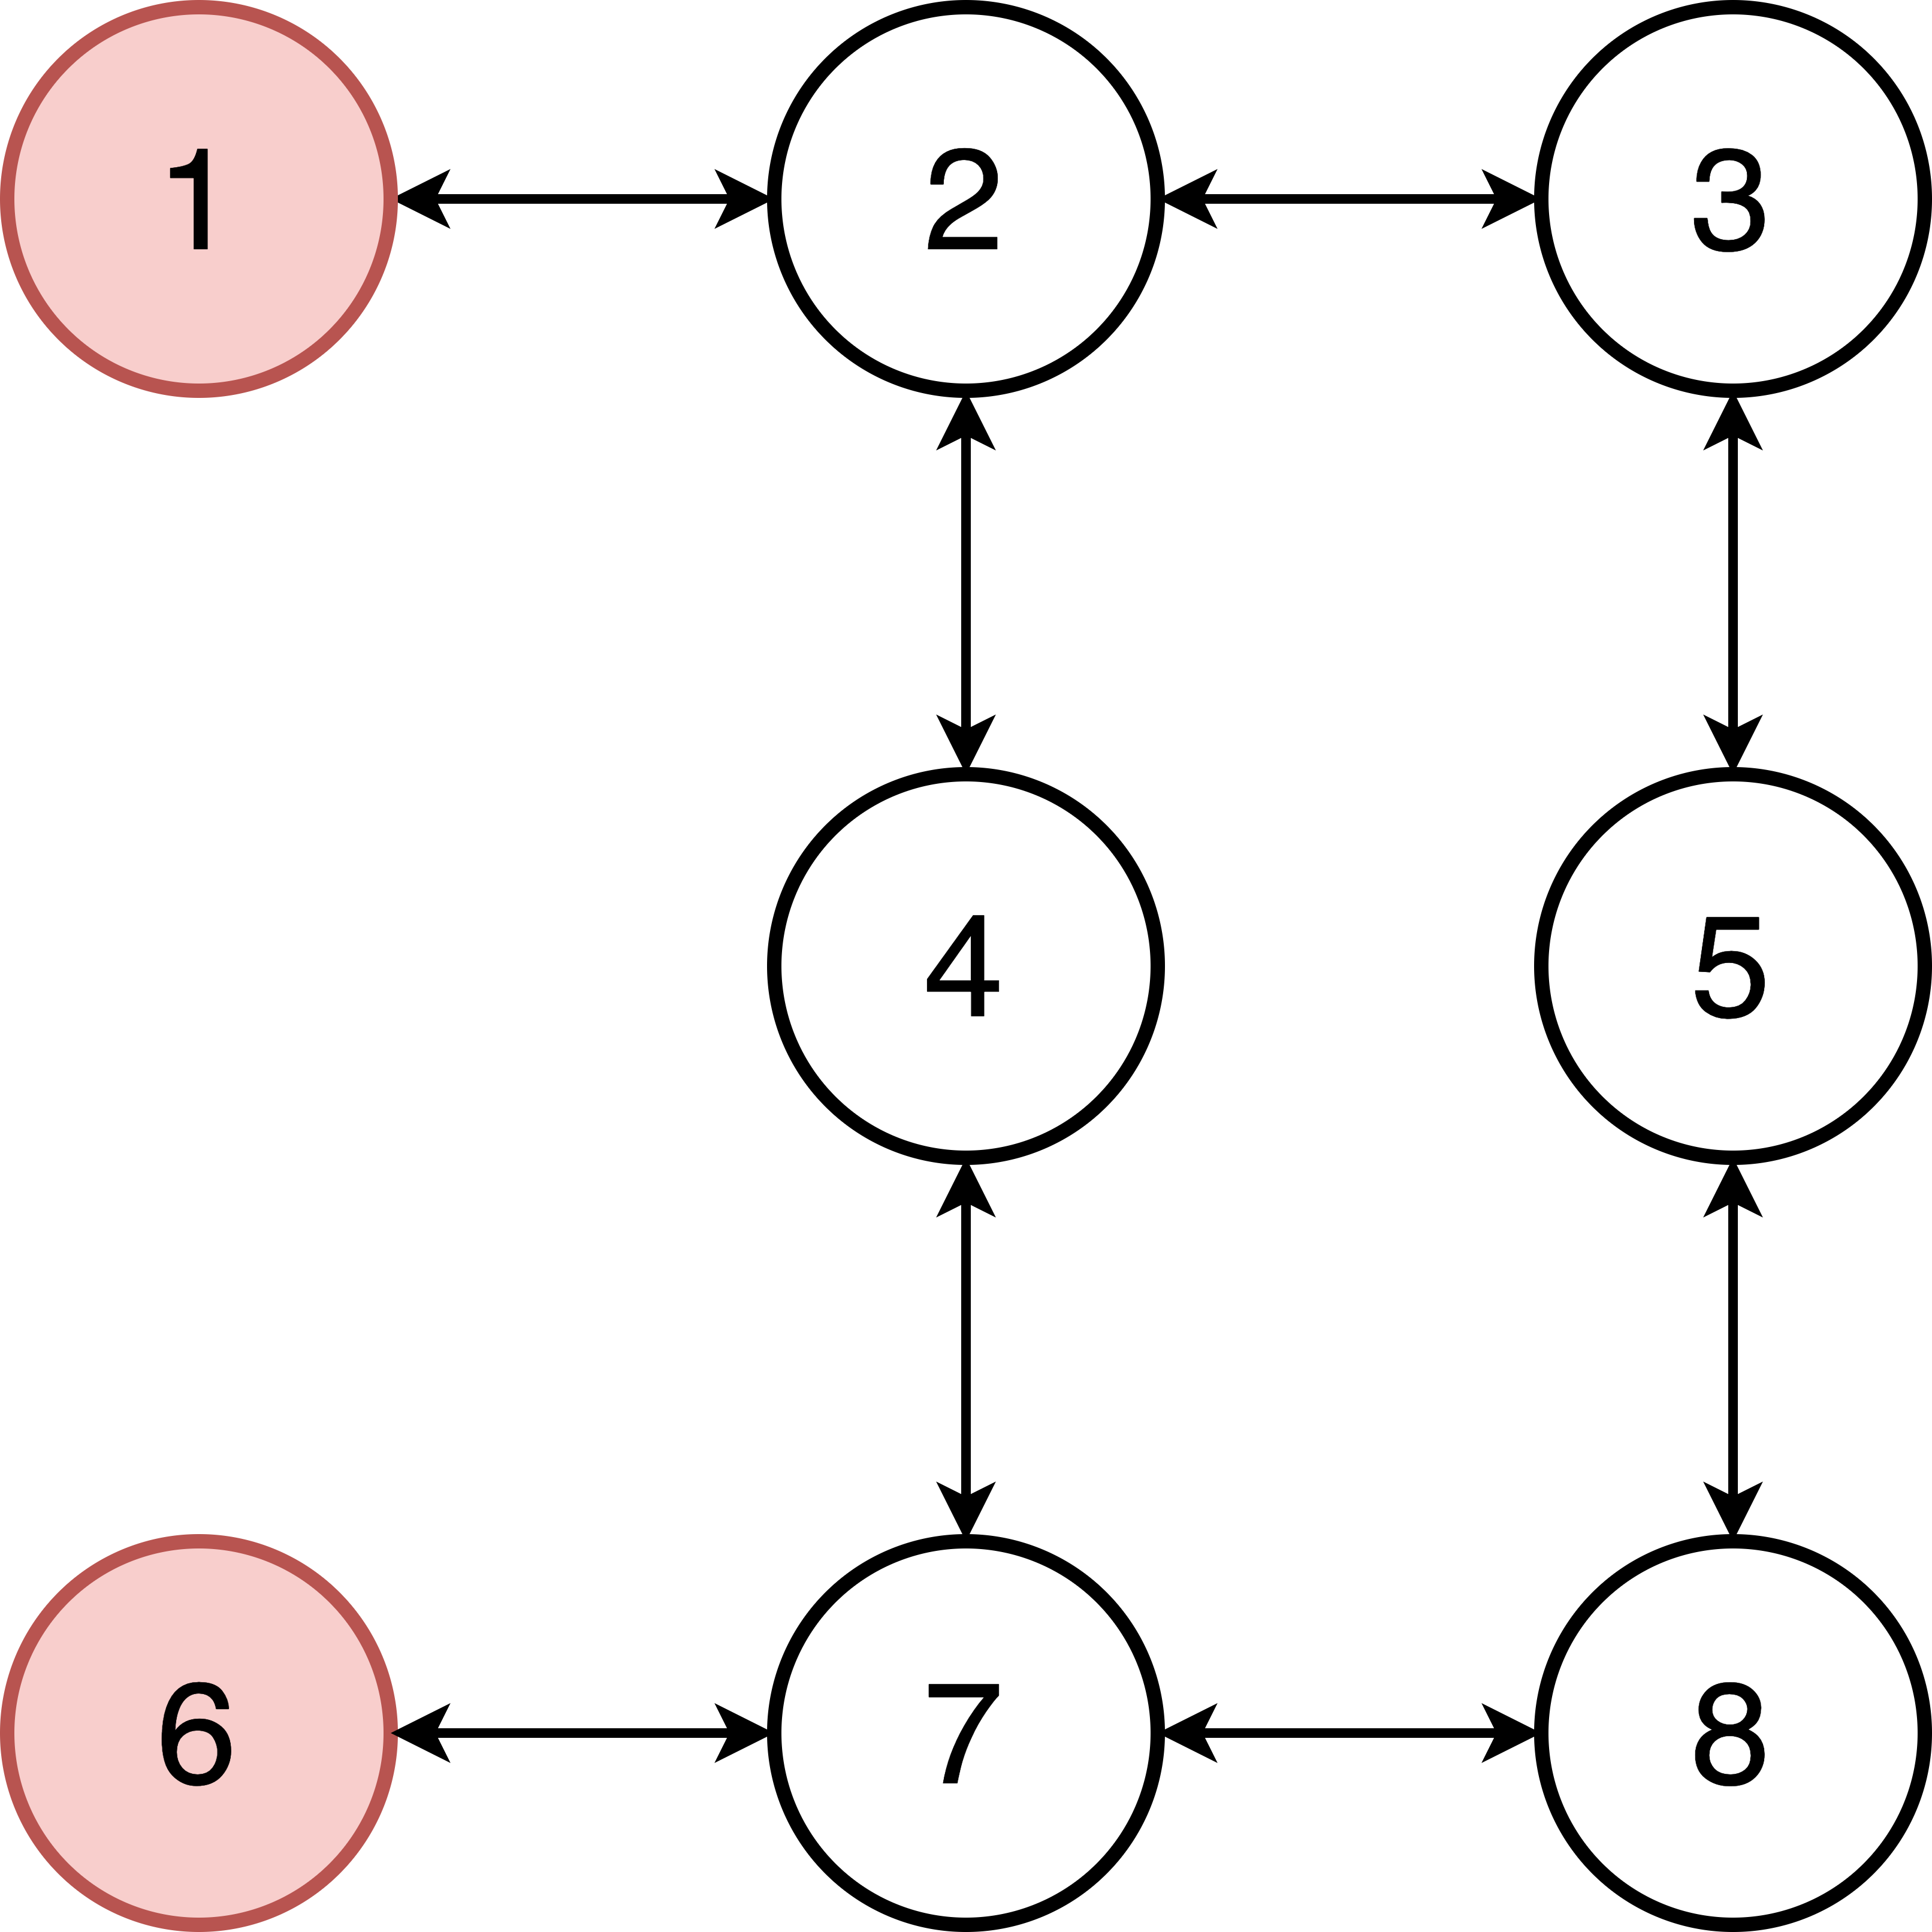
\includegraphics[width=0.35\linewidth]{STExample}
  \caption{A possible example a \acrs{SAPF} problem that the low-level search
  must solve. The agent starts from vertex 1 and has to reach vertex 6.}
  \label{fig:STExample}
\end{figure}
The main problem that this algorithm aims at solving raises from an observation
of the difficulty in finding alternative paths when faced with constraints. For
example, consider Figure~\ref{fig:STExample}: it is possible to follow two
paths to go from vertex 1 to vertex 6:
\[
  \begin{array}{l}
    \pi_1 = \{1,2,4,7,6\}\\
    \pi_2 = \{1,2,3,5,8,7,6\}
  \end{array}
\]
Obviously, the second path is longer than the first one and it would never be
selected if the first could be used. Let's suppose though that the agent cannot
be on node 4 at times 3 and 4, then the two paths start to have the same 
length. \newline
\milc{spanningTree} provides alternative paths in an easy way, so that the
low-level search may select the best to pass to the high-level search. The
algorithm works as described in Algorithm~\ref{algo:ST}.
\begin{algorithm}[htb]
  \DontPrintSemicolon
  \caption{The pseudo code for the spanning tree algorithm}
  \label{algo:ST}

  \KwIn{\texttt{nodes}: the list of nodes}
  \KwIn{\texttt{initPos}: the initial position}
  \KwIn{\texttt{endPos}: the final position}
  \KwIn{\texttt{goalPos}: the list of goal positions}
  \KwIn{\texttt{connect}: the connectivity matrix}
  \;
  \KwData{\texttt{finalPaths}: a vector containing the paths that are valid}
  \;
  \Begin{
    \If{\texttt{goalPos} is empty}{
      \Return \texttt{spanningTreeP2P} between \texttt{initPos} and
      \texttt{endPos}\;
    }
    \Else{
      \texttt{start} $\gets$ \texttt{initPos}\;
      \texttt{end}   $\gets$ \texttt{goalPos[0]}\;
      Insert the solution of \texttt{spanningTreeP2P} from \texttt{start} to
      \texttt{end} in \texttt{finalPath}\;
      \For{Each remaining goal in \texttt{goalPos}}{
        \texttt{start} $\gets$ \texttt{end}\;
        \texttt{end}   $\gets$ next goal\;
        Insert the solution of \texttt{spanningTreeP2P} from \texttt{start} to
        \texttt{end} in \texttt{finalPath}\;
      }

      \texttt{start} $\gets$ last goal\;
      \texttt{end}   $\gets$ \texttt{endPos}\;
      Insert the solution of \texttt{spanningTreeP2P} from \texttt{start} to
      \texttt{end} in \texttt{finalPath}\;
    }
  }
\end{algorithm}\newline
The point-to-point spanning tree function \milc{spanningTreeP2P} works in the
following way:
\begin{enumerate}
  \item Initialize a set of nodes (\texttt{OPEN}) to be explored with their
    distance from the source and a list of paths (\texttt{paths}).
  \item Initialize the distance of the first node.
  \item Start from the source, add to \texttt{OPEN} all the neighbors of the 
    source increasing the distance by one. 
  \item Then until \texttt{OPEN} has elements, pop the last element from the
    list and iterate with the same procedure as for the root adding the
    neighbors of the considered node to \texttt{OPEN} and adding each
    considered node to the current path. 
  \item At each iteration, the following checks are carried out:
    \begin{itemize}
      \item If the element that was popped is the arrival node, then the path
        we have found until now is valid and can be stored.
      \item If the considered node is already inside the path, then the path is
        a cycle and should not be considered, discard the path.
      \item If the distance of the current node is less than the distance of
        the last node added to the path, then the path is not valid, should be
        dropped and the new node should be added to the path.
    \end{itemize}
    Each time one of the conditions is true, either the path is dropped or it
    is stored. In the latter, a new path is added to \texttt{paths} starting
    from the last node that had more than one neighbor added to \texttt{OPEN}.
    When the former happens instead, the path is not added to \texttt{paths},
    but we erase all the nodes up to (and excluded) the node that generated
    more neighbors in \texttt{OPEN}. To check which node is the one responsible
    for multiple neighbors, we check the last distance in \texttt{OPEN} and the
    position of the node to be erased inside its path. 
  \item When \texttt{OPEN} is empty, then we can return. Before returning we
    check if the last path that was being built has reached the final
    destination and if it has not, then it is removed from the list. 
\end{enumerate}
Another key aspect is how to merge the point-to-point paths to obtain a single
path. Indeed this is a weak spot of the proposed algorithm since it is actually
a combinatorial problem which may cause the memory usage to raise
exponentially. Indeed, for every \texttt{spanningTreeP2P} invocation after the
first, the previous vector of solutions is copied as many times as the number
of the new solutions and each one of the solutions is added to the old ones.
\newline
The algorithm so described works for solving a \acrs{sapf} problem with the
addition of intermediate goals and it returns a vector of possible paths to
reach the destination while passing through the goals. We now need to also 
consider the possible constraints from high-level. To do this, we first order
the constraints following a temporal order, then we iterate through the paths 
and check whether a given path violates one or more constraints. If it does,
then we insert a copy of a safe node to indicate that the agent must stay on
the previous node to avoid the conflict. Finally, once we have gone through all
the paths and fixed the possible conflicts, we are going to return the shortest
path to the high-level search. \newline
The important point of this problem is how to choose a "safe" location.
Initially, the safe location is the starting node, i.e., index 0, then each
time a constraint is fixed, the safe location moves to the time of the
constraint. This allows to produce a path that is free from collisions. Notice
that it is important that the constraints are temporally ordered, otherwise
adding nodes in which the agent should stay may produce other violations. 
%
\subsubsection{\acrf{TDSP}}
\label{ssec:tdsp}
This low-level search is mainly based on the algorithm from 
Dijkstra~\cite{dijkstra}, but we introduce a new structure to handle the edges 
between nodes. \newline
This structure is trivially named \texttt{Connection} and stores two important 
pieces of information:
\begin{itemize}
  \item The type of connection, which can either be:
    \begin{itemize}
      \item \texttt{ONE}: when the edge is always valid;
      \item \texttt{ZERO}: when there is never an edge between two nodes;
      \item \texttt{LIMIT\_ONCE}: when the connection is always valid except for
        the specified time step(s);
      \item \texttt{LIMIT\_ALWAYS}: when the connection is never valid except
        for the specified time step(s).
    \end{itemize}
  \item A vector of time steps, which can either be times in which the edge
    should not be considered, or times in which the edge is valid. 
\end{itemize}
Before calling the shortest path algorithm, the low-level search transforms the
connectivity matrix from integer values to objects of time \texttt{Connection}
taking into consideration the constraints. This allows the algorithm to avoid a
path if the edge is not valid in that time step as it would lead to a vertex or
a swap conflict. \newline
This alone though may not solve the problem, i.e., find a feasible path given
the constraints, as all it does is stating that the agent should or not use a
certain edge. In order for the agent to stay on a node, we need to add a
virtual node, which we will refer to as placeholder. What the algorithm does is
to see that at a given time $t$ the agent cannot be on a node $n$, then it adds
a placeholder for the node, it limits the connections of all the nodes that
previously had a valid connection to the node $n$ at time $t$ and replaces this
connections with a valid connection to the placeholder only for time $t$. This
basically increases the path length of one unit and during the phase of
post-processing it is possible to remove the placeholder and add a node where
the agent can stay. \newline
Instead, we consider swap conflicts as a double vertex conflict: if a node 
cannot go from a node $n_i$ to a node $n_j$ at time $t$, this means that at
time $t+1$ it can neither be on $n_i$ since it will be occupied from the other
node, nor on $n_j$ since it would cause a swap conflict. \newline
The rest of the shortest path algorithm is dealt with in the following way:
\begin{itemize}
  \item Compute the shortest path between the initial point and the first goal
    point; 
  \item Iterate between the various goal points in list;
  \item Compute the shortest path between the last goal point to the final
    vertex.
\end{itemize}
The so obtained path is the shortest path (assuming correctness and optimality
of the chosen shortest path algorithm) that meets all the goals and respects
the constraints. In our case, the shortest path algorithm is the Dijkstra's 
algorithm which is optimal unlike \astar that must prove that the used
heuristic is admissible to be optimal.
%
%
\subsection{High-Level Search}
The high-level search is basically the same as the one described in
Section~\ref{ssec:cbs}. We start from a root node which does not contain any
constraint and we compute the best path for each agent considering the agent as
if it was in \acrs{sapf} problem. Then we check for conflicts:
\begin{itemize}
  \item if no conflict was found, then this is the solution to return;
  \item if a one or more conflicts were found, then only the first conflict is
    considered. 
\end{itemize}
To check for conflicts, we compare each path with all the other paths. Each
element in the vector representing the path corresponds to the node occupied by
an agent at a certain time $t$, so the indexes of the vector correspond to the
time steps. So when a vertex conflict is found, it happens because at the same
index, both vectors have the same node, while when a swap conflict is found
then the node of a vector at index $t$ corresponds to the node at index $t+1$ 
of the other vector and vice versa. \newline
When a conflict is found, two constraints are produced:
\begin{itemize}
  \item Vertex conflict: in one constraint, agent $a_i$ cannot be on node $n$
    at time $t$, on the other constraint, agent $a_j$ cannot be on node $n$ at
    time $t$.
  \item Swap conflict: in one constraint, agent $a_i$ cannot go from node $n_1$
    to node $n_2$ at time $t$, on the other constraint, agent $a_j$ cannot go
    from node $n_2$ to node $n_1$ at time $t$. 
\end{itemize}
For each constraint, the low-level search is called: since the constraint
affects only one agent, then only its path is going to be recomputed. If the
low-level manages to find a solution, then the high-level adds a new node with
the new solution and also adds the constraint to the constraints list of the
new node. The search is repeated until a valid solution is found. 
%TODO talk about how to move from weighted edges to unitary edges
